\documentclass{beamer}
\usepackage{geometry, amsfonts, amsmath, tikz, multicol, tikz-imagelabels, 
            multirow, pifont, xcolor, tcolorbox}

\usetheme{Madrid}

\setbeamertemplate{frametitle}[default][center]
\usecolortheme{dove}
\title [BAC Discussion]{ BAC Discussion}
\author[Maria Jose]{Maria Jose}
\date{\today}
\institute[UVA]{University of Virginia}
\hypersetup{
    colorlinks=true,
    linkcolor=cyan,
    filecolor=magenta,      
    urlcolor=cyan,
    pdftitle={Overleaf Example},
    pdfpagemode=FullScreen,
    }

\definecolor{uvablue}{RGB}{35,45,75}
\definecolor{uvaorange}{RGB}{229,114,0}
\definecolor{UniBlue}{RGB}{83,121,170}
\definecolor{forestgreen}{RGB}{0,128,0}
\definecolor{bronze}{rgb}{0.8, 0.5, 0.2}
\definecolor{purple}{RGB}{128,0,128}
\definecolor{maroon}{RGB}{184,15,10}
\definecolor{grey}{RGB}{128,128,128}
\definecolor{bondiblue}{rgb}{0.0, 0.58, 0.71}
\definecolor{gold}{RGB}{160,116,10}
\definecolor{peacockblue}{RGB}{0,164,180}

%\setbeamercolor{frame}{bg=black, fg =white}
%\setbeamercolor{frametitle right}{bg=gray!60!white}
%setbeamercolor{palette primary}{bg=black,fg=white}
\setbeamercolor{structure}{fg=uvaorange}
\setbeamercolor*{frametitle}{ fg =peacockblue}
\setbeamercolor*{title}{ fg = peacockblue}
%\setbeamercolor{alerted text}{fg=red!85!black}
\setbeamercolor*{palette primary}{fg =peacockblue}
\setbeamercolor*{palette secondary}{fg =peacockblue}
\setbeamercolor*{palette tertiary}{fg =peacockblue}
\setbeamercolor*{palette quaternary}{fg =peacockblue }
%\setbeamercolor*{background canvas}{bg=uvablue}
%


%\setbeamercolor*{block body}{fg=black,bg=black!10}
%\setbeamercolor*{block title alerted}{,bg=black!15}
%\setbeamercolor*{block title example}{parent(0,164,180)=example text,bg=black!15}

\imagelabelset{
coordinate label font = \sffamily\bfseries\tiny,
coordinate label distance = 1mm,
coordinate label back = white ,
coordinate label text = uvaorange,
annotation font = \normalfont\tiny,
}
%\logo{%
%  
% 
\includegraphics[width=1cm,height=1cm,keepaspectratio]{../Universitylogos/CMSlogo.png}%
%  \hspace{\dimexpr\paperwidth -2cm}%
% \vspace{\dimexpr\paperwidth }%
% 
\includegraphics[width=1cm,height=1cm,keepaspectratio]{../UniversityLogos/rotunda.jpg}%
%
%}

\begin{document}

\maketitle
\begin{frame}{Assembly Status}
\begin{itemize}
    \item We have assembled 480 SMs and QA/QCed 432 with the Cesium source.
    \item Last week we had two 24 SM assembly days.
\end{itemize}
\centering
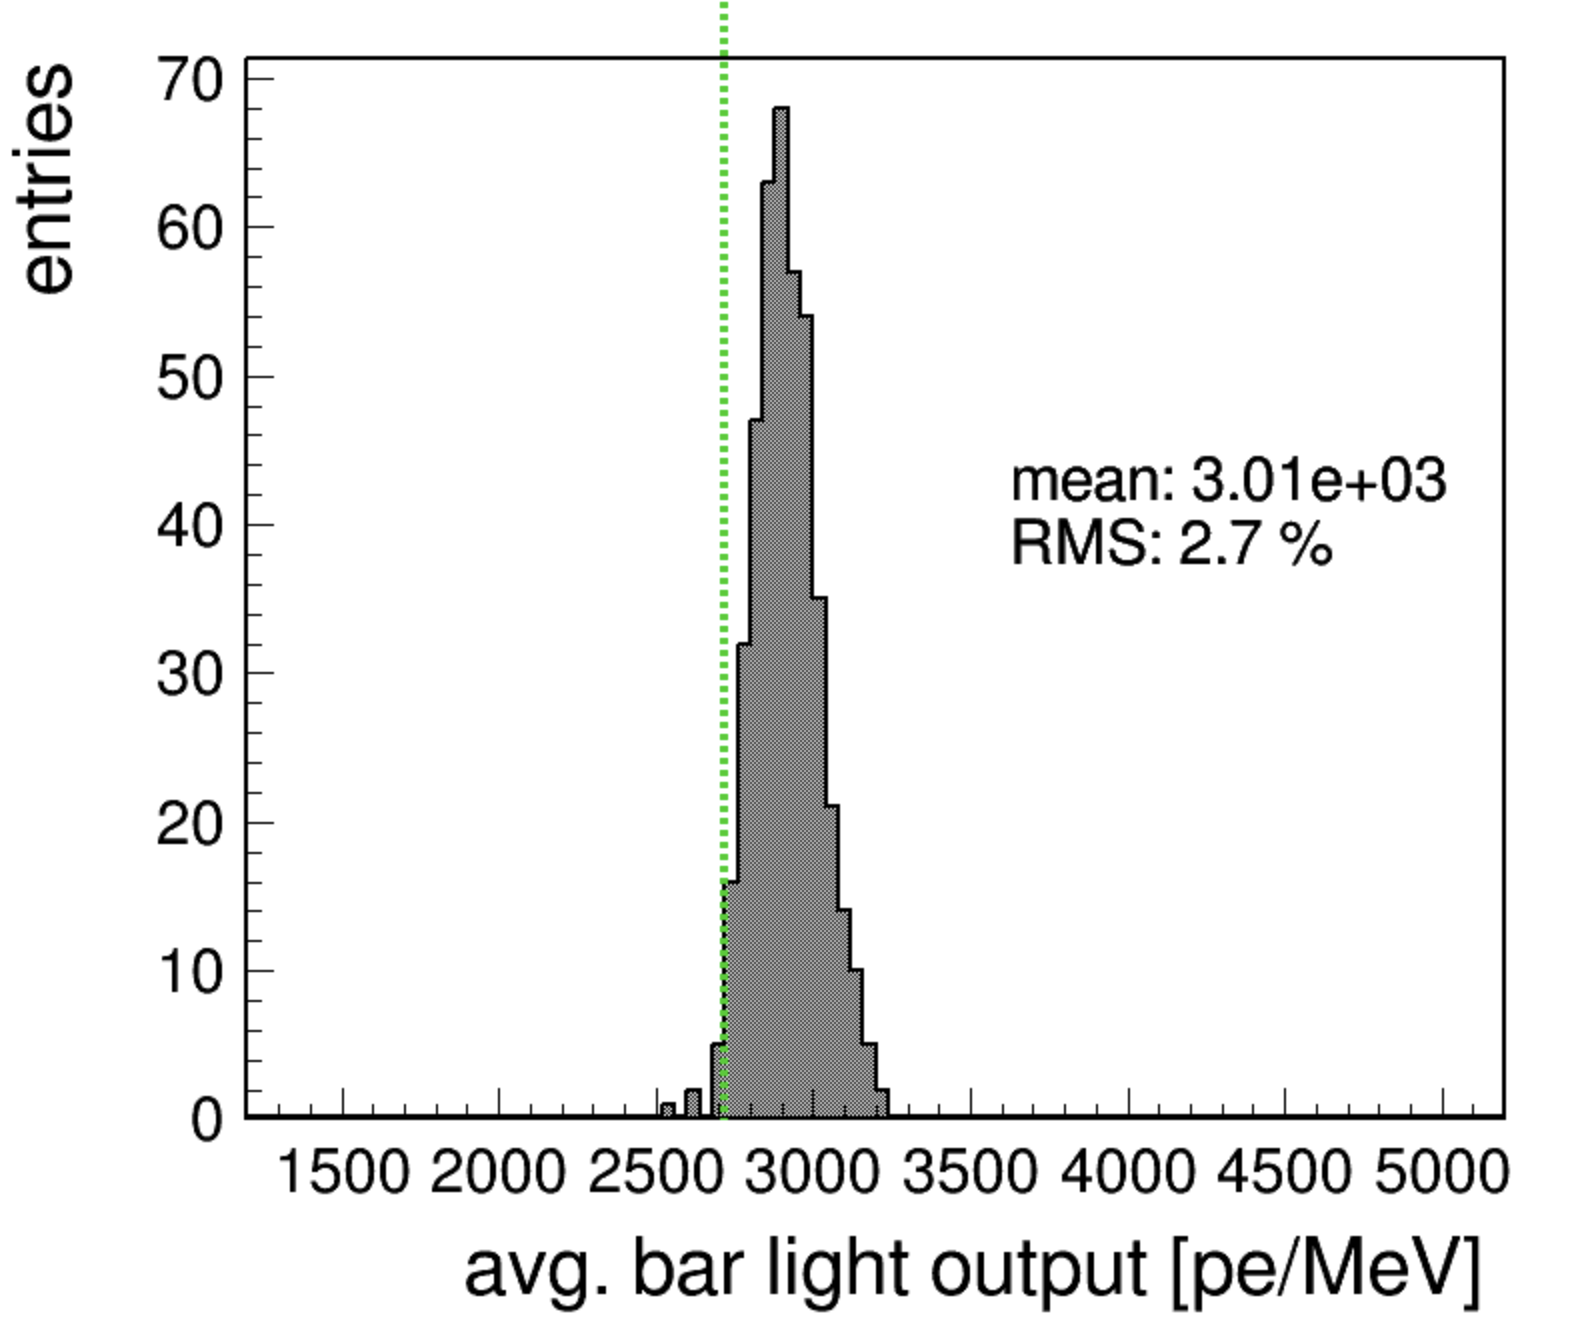
\includegraphics[width=5cm, height=5cm]{../btl_files/summary_plots/summary_432.png}
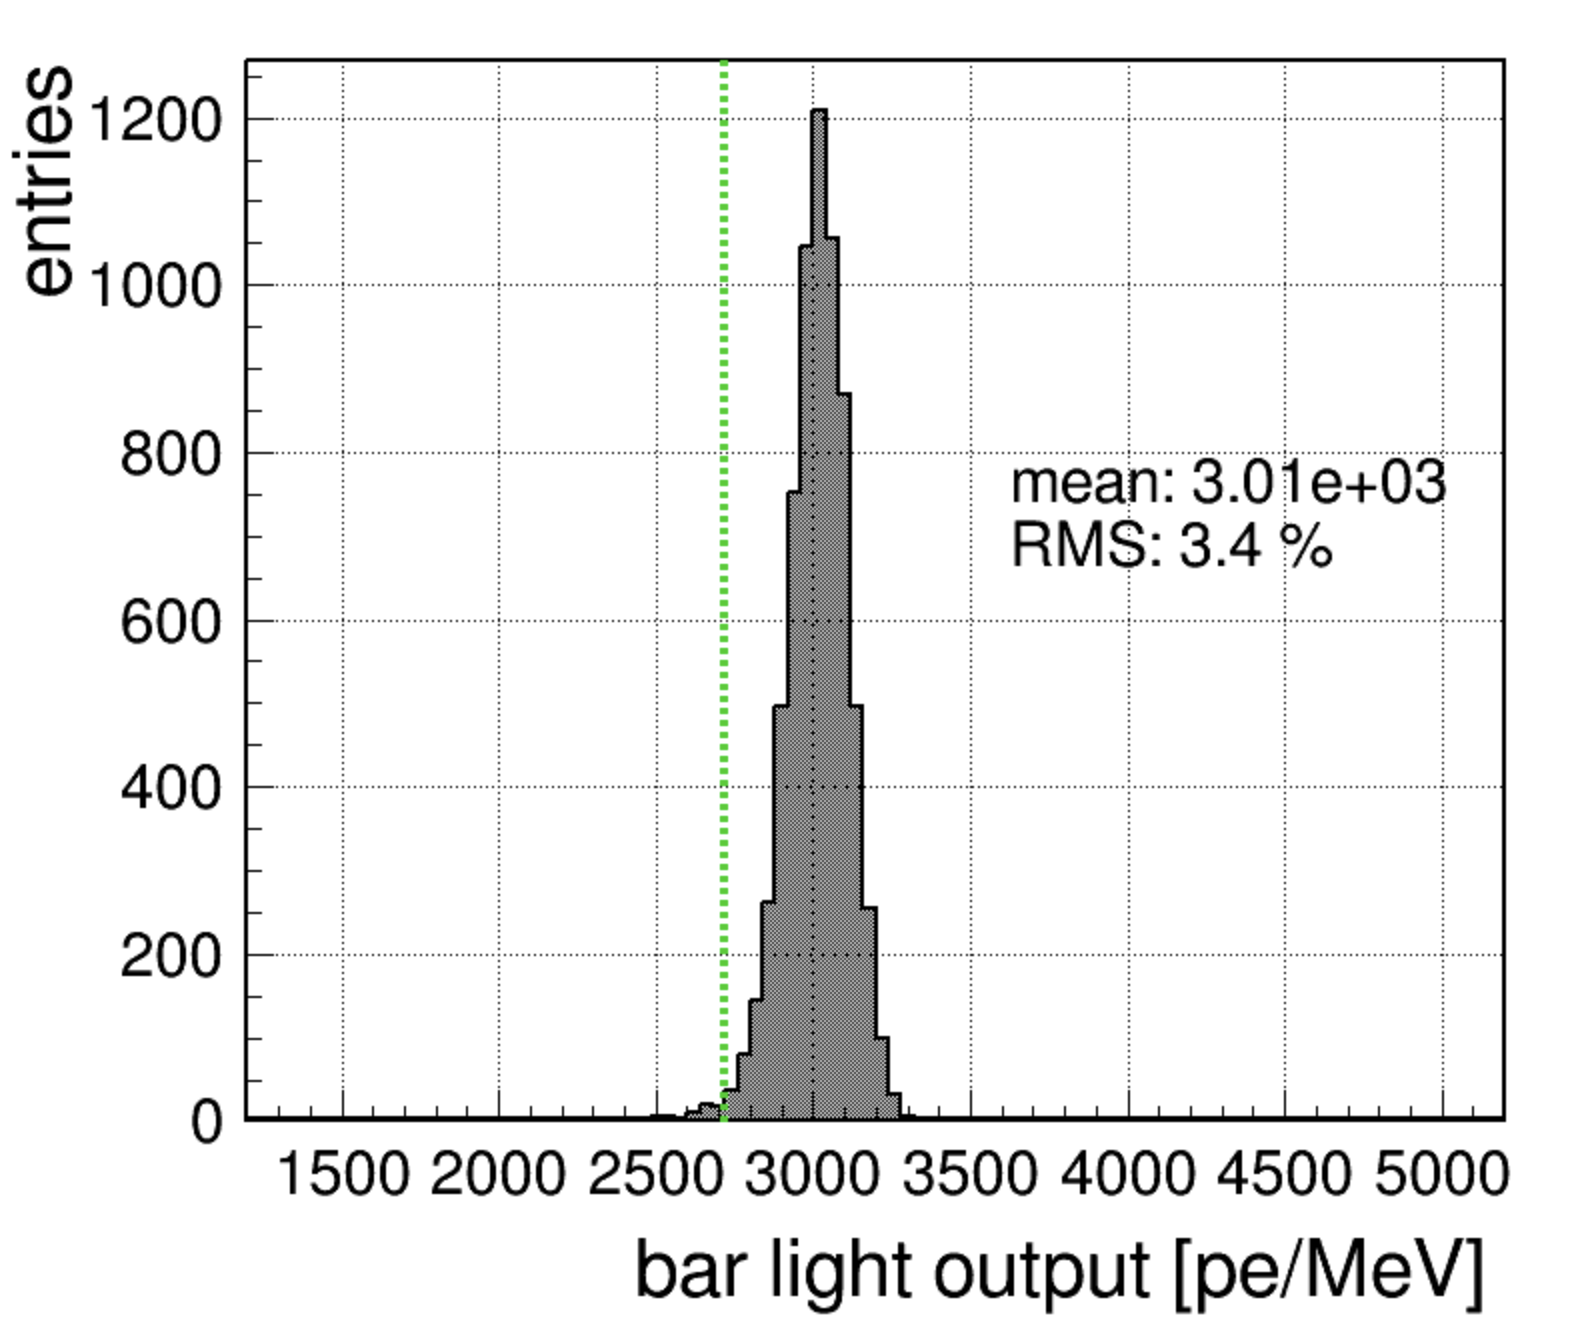
\includegraphics[width =5cm, height =5cm]{../btl_files/summary_plots/summary_432_ch.png}
\end{frame}
\begin{frame}{Offset Correction}
After we changed DC offeset from 28500 to 22000, we don't see the saturation of the pulses anymore.\\
\centering
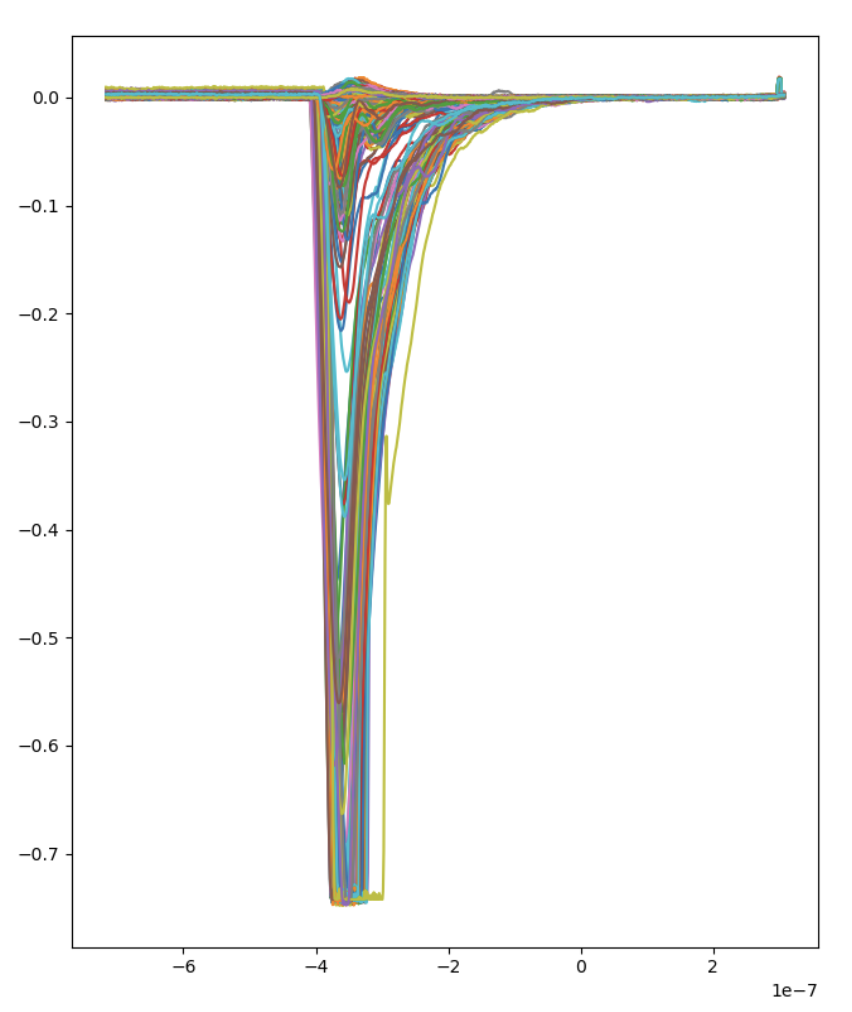
\includegraphics[width=4cm, height=4cm]{../btl_files/offset_plot/without_offset.png}
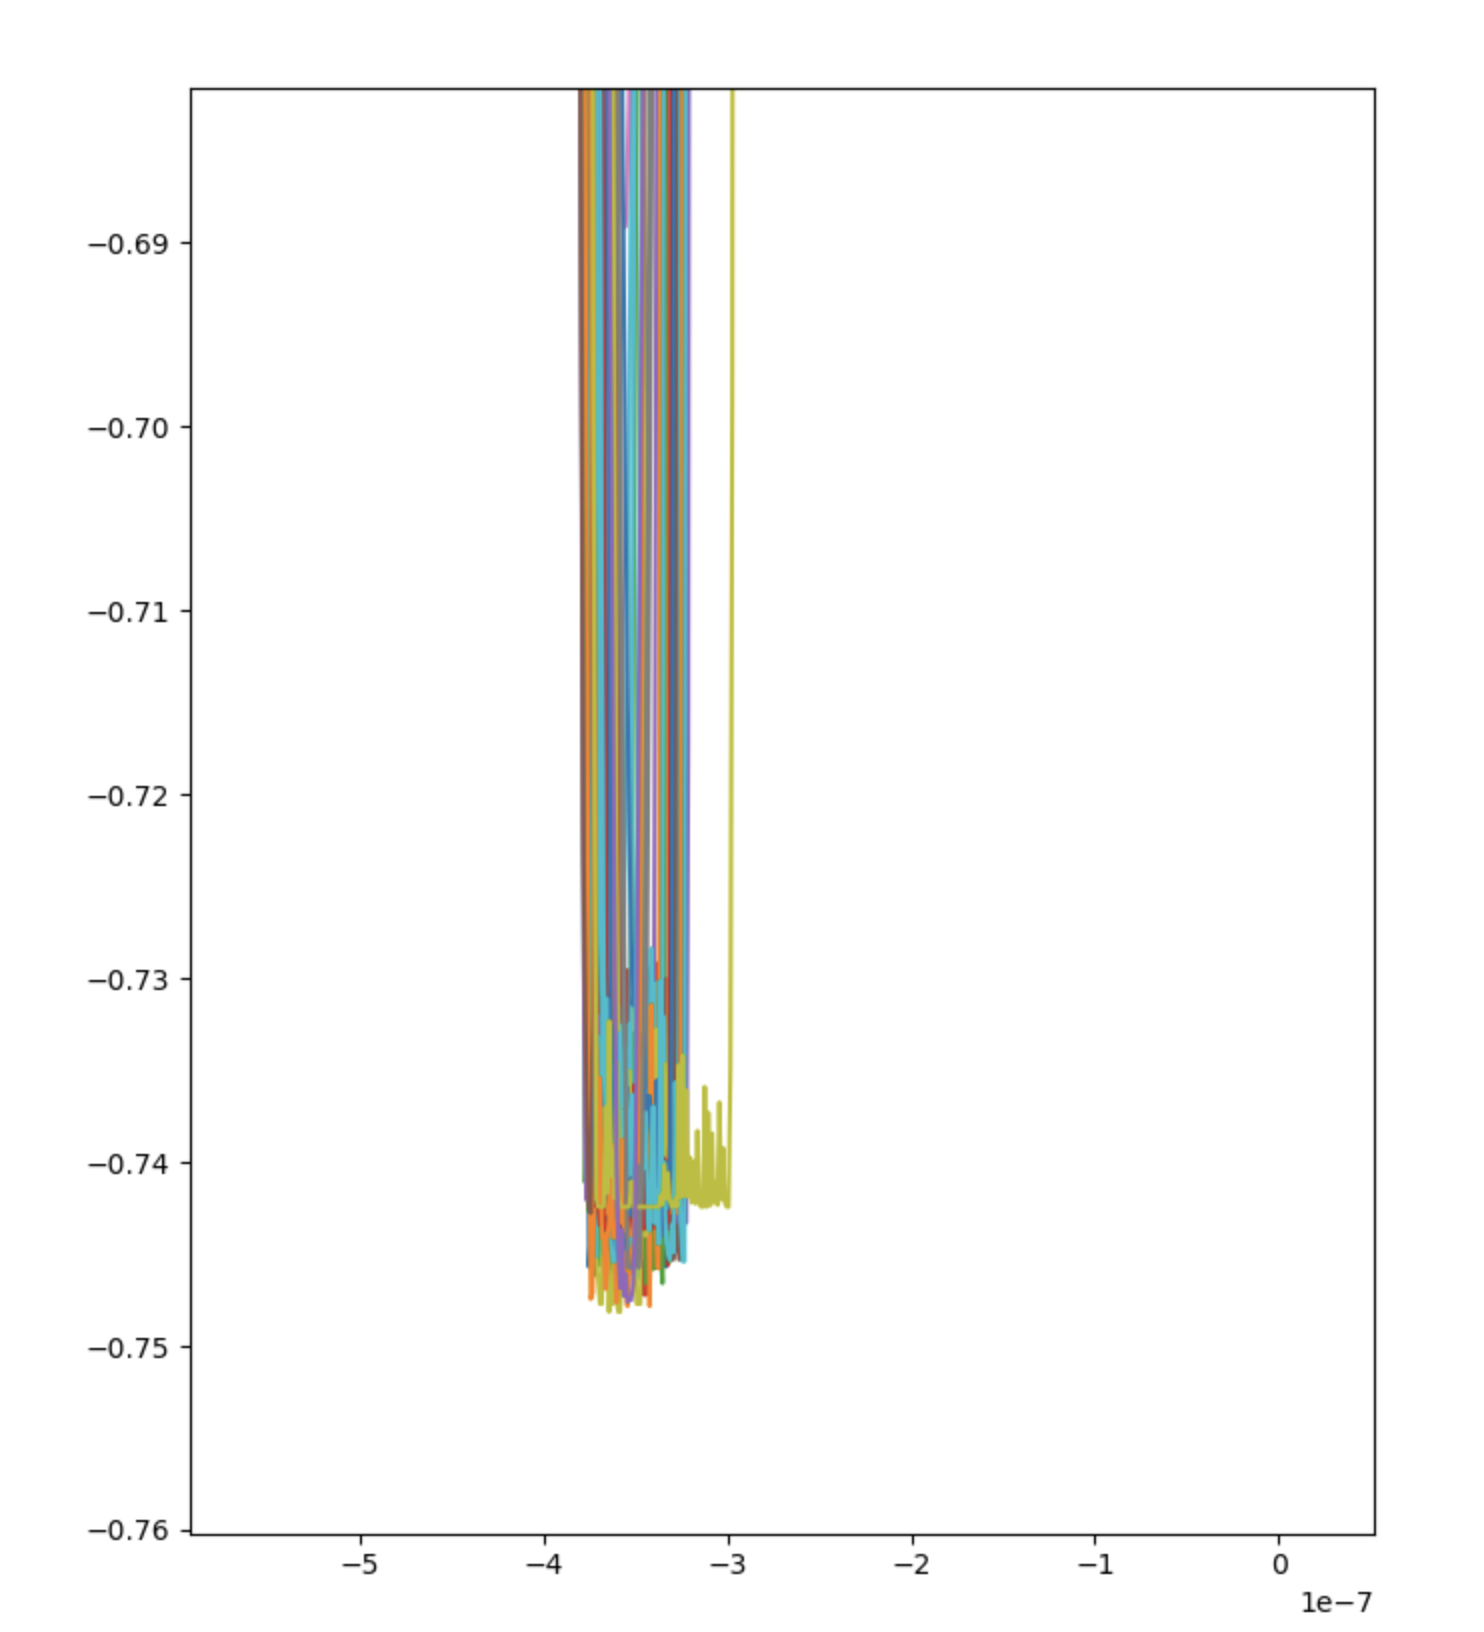
\includegraphics[width=4cm, height=4cm]{../btl_files/offset_plot/without_offset_zoom.png}\\
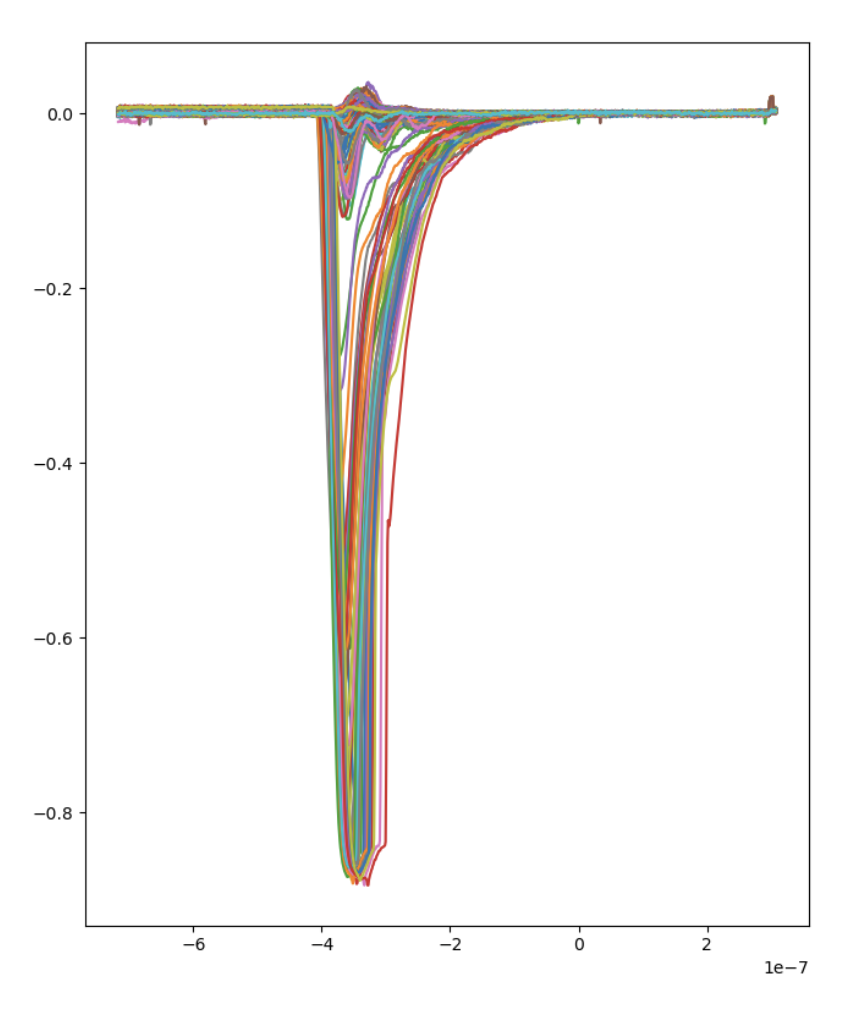
\includegraphics[width=4cm, height=4cm]{../btl_files/offset_plot/with_offset.png}
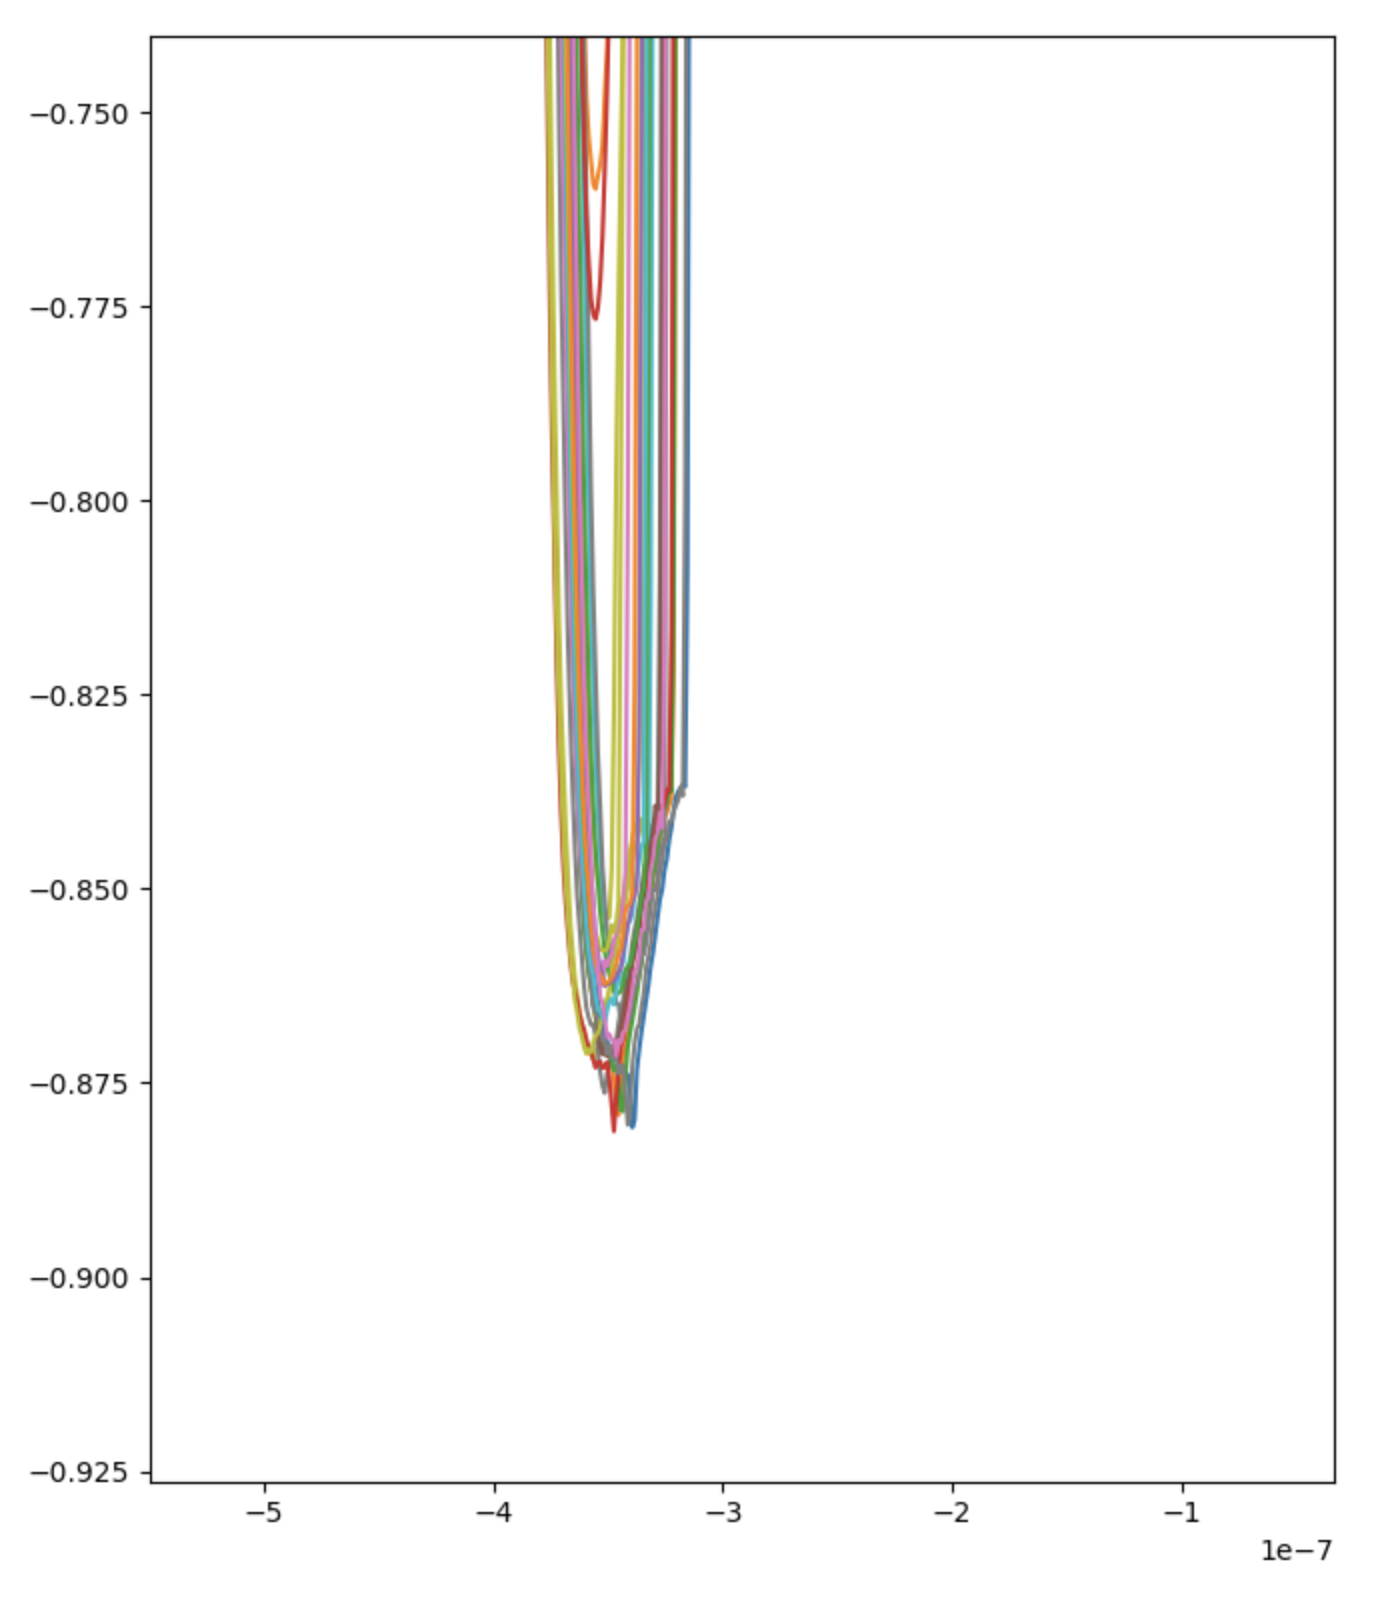
\includegraphics[width=4cm, height=4cm]{../btl_files/offset_plot/with_offset_zoom.png}\\
\end{frame}
\begin{frame}
\frametitle{Taking Data with Sodium Source}
\begin{itemize}
    \item We have tried taking data with the Sodium source and we could get the fit working for all the channels.
    \item Already made the changes Andrea suggested to do.
\end{itemize}
\centering
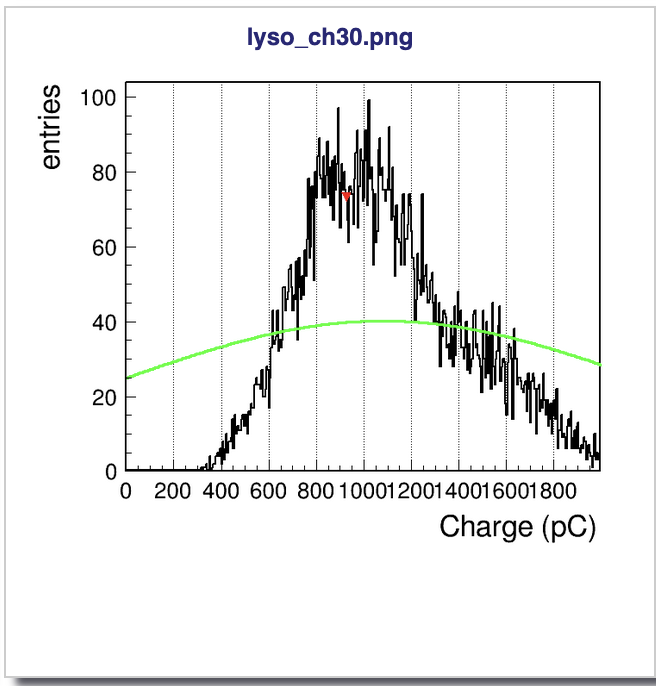
\includegraphics[width=5cm, height=5cm]{../btl_files/sodium_fit_fail/Screenshot 2025-01-26 at 10.59.21.png}
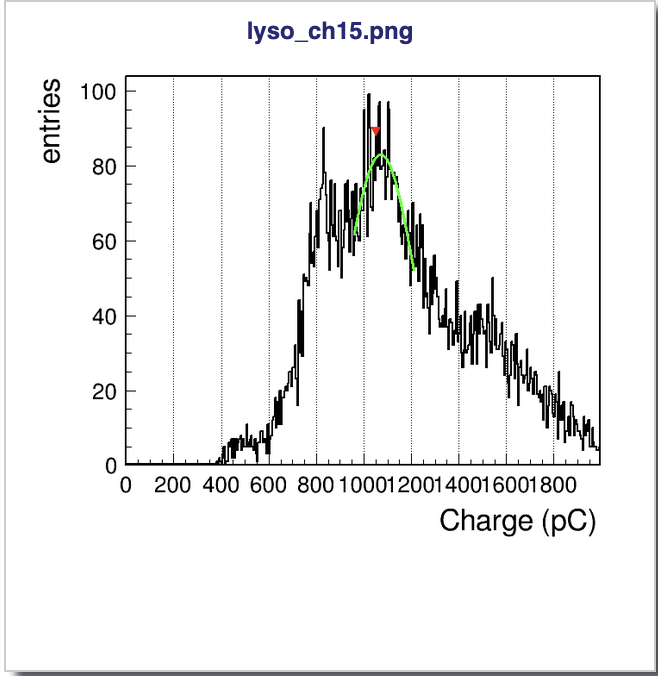
\includegraphics[width=5cm, height=5cm]{../btl_files/sodium_fit_fail/Screenshot 2025-01-26 at 10.59.34.png}
\end{frame}
\end{document}